\documentclass[a4j,12pt, twocolumn]{jarticle}
\usepackage[dvipdfmx]{graphicx}
\usepackage{amssymb}
\usepackage{amsmath}
\usepackage{float}
\usepackage{slashbox}
\usepackage[compact]{titlesec}
%---------------------------------------------------
% ページの設定
%---------------------------------------------------
\setlength{\textwidth}{170truemm}
\setlength{\textheight}{255truemm}
\setlength{\topmargin}{-14.5truemm}
\setlength{\oddsidemargin}{-5.5truemm}
\pagestyle{empty}
\setlength{\headheight}{0truemm}
\setlength{\parindent}{1zw}

\begin{document}
\twocolumn
[
\begin{center}
  {\huge NAISTにて取り組みたい研究について}
\end{center}
\begin{flushright}
\begin{tabular}{ll}
氏名: & 新妻巧朗\\
試験区分: & 情報科学区分\\
希望研究室: & 自然言語処理研究室\\
\end{tabular}
\end{flushright}
\vspace{2truemm}
]
\section{はじめに}
\subsection{NAISTで取り組みたいこと}
 NAISTにて、私が取り組みたい研究テーマは「情報検索システムにおける検索質問に合わせた適切なファセットの推薦、およびファセットの自動生成手法について」である。
\subsection{これまでの修学経験}
 これまでは、地方の産業構造に関する実証分析について研究してきた。特に卒業研究では総生産と地域を構成する産業に着眼し、経済格差が生じる要因について分析をした。

\section{研究の概要}
\subsection{背景・社会的意義}
 現代社会において情報収集をするためには、検索エンジンを利用することは必要不可欠である。しかし、検索エンジンを適切に活用できず、目的の情報に至れない場面も多い。それは多くの検索エンジンの仕組みが、利用者に対して情報検索能力を要求しているからである。これまでも福島らの研究にて情報検索能力は個人差が大きく、能力差によって情報格差が生じていることが調査されてきた\cite{fukushima}。

 こうした課題を解決することで、情報に辿りつけないことで生じる機会損失を減らすことができるのではないかと考えている。
 
 過去に齋藤らによる教育を通して情報検索能力を向上させる研究\cite{saito}も存在しているが、本研究ではシステムの拡張によって解決するアプローチを考えていく。

 福島らによって言語能力の高さが情報検索能力に高さに関係しているとわかっている\cite{fukushima}。つまり、言語能力の高低が情報検索における情報格差を生み出していると考えられる。そのため、情報の探索過程で言語能力を要求する場面にて利用者の補助をおこなうシステムを提案したい。
\subsection{提案内容}

 そこで、利用者が入力した検索質問に対して適切なファセットを推薦し、インクリメンタルに検索意図を読み取るシステム(図1)を提案したい。

 \begin{figure}[h]
   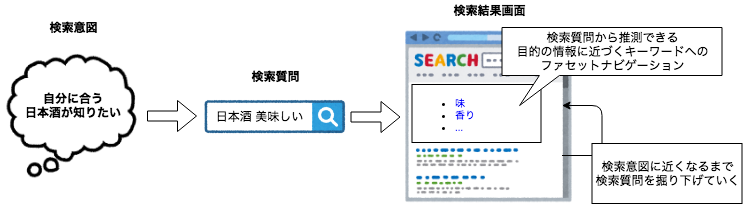
\includegraphics[width=85mm]{./new_ir_with_navi.png}
   \caption{システムのイメージ図}
 \end{figure}
 
 情報の探索行動を掘り下げると、検索意図と検索対象の意味的な距離を縮めていくプロセスと考えられる。 そのため、ファセット検索という手法が役に立つのではないかと考えた。ファセット検索とは、検索システムの利用者に検索対象を何らかの側面で絞り込むファセットを提示し、検索対象を絞り込む検索手法である\cite{faceted}。これは、システムの利用者が検索意図を掘り下げて言語化する行動をシステムが代行していると言える。そのため、検索エンジンが個人の言語能力に依存している問題にアプローチできると考えている。
\section{研究の展望}
 先に提案したシステムを実現するためには、検討しなければならない課題が二つある。
\begin{enumerate}
  \item 検索質問に対応するファセットを提示する方法
  \item 索引対象から最適なファセットを推測して生成する方法
\end{enumerate}

 前者の課題については、膨大な量のファセットをそのまま提示したのでは、利用者の負担が増えるだけであるためだ。Webのような膨大な数の文書が存在する空間を対象とした場合、文書の種類も無数に存在する。その結果、文書を分類することで作成されるファセットの数も同様に膨大な数になり、利用者が絞り込める数ではなくなってしまう。そのため、検索質問に合わせて関連したファセットを推薦することで解決をしたいと考えた。つまり、検索質問から関係するファセットを得る必要がある。検索質問は文書内のキーワードと一致することを念頭に入力されたものであると考えられるため、検索質問は文書内の語彙と同一視することができる。そこから、検索質問とファセットの関係性は、索引対象の語彙間の関係性を抽出することで擬似的に取得できると考えられる。

 後者の課題については、索引対象がWebのように膨張しつづけている場合、ファセットの作成を従来の手段に頼ることが難しいためである。従来のファセット検索ではシステムの提供者が索引する文書から属性データを作成する必要があった。しかし、Webでは文書の種類も日々増え続けており、文書の属性データの作成を人の手で対応していくことは現実的でない。そこで生成可能な属性データを推測してファセットを自動的に生成することで、この課題を解決しようと考えた。ファセットは語彙の上位下位のような関係性によって定義される。そのため、実現には索引対象から語彙間の関係性を抽出することが必要である。

上記の課題の解決手段として、ともに語彙間の関係性を抽出することの必要性を述べた。これまで語彙同士の関係性を抽出する研究は、情報抽出の領域におけるbankoらによる研究\cite{banko}を皮切りに、 OpenIE(Open Information Extraction)という分野にて研究されてきた歴史がある\cite{niklaus}。これらの研究成果を活用して、先に挙げた課題に対応する手段を検討していきたい。

\section{まとめ}
ここまで私がNAISTにて取り組みたい研究テーマについて述べた。

 これまでソフトウェアエンジニアとしてWebサービスに携わる中で、検索システムの利用者が得たい情報をどのように探索しているのか、どうあると嬉しいのかについて考えてきた。特に現在携わっているアルバイト求人のデータベースメディアでは、サイトの利便性の向上のために、どのようにファセットナビゲーションを実現するとよいか、求人検索機能のファセットナビゲーションをどのように実装すべきかなどを試行錯誤する機会に恵まれた。こうした経験が本研究には役立つのではないかと考えている。

\begin{thebibliography}{9}
\bibitem{fukushima}
   福島健介・小原 格・須原慎太郎・生田 茂(2005), インターネット検索能力の差異に及ぼす 要因の検討 その1, コンピュータ&エデュケーション VOL.18 2005
\bibitem{saito}
   齋藤ひとみ・三輪和久(2004),  Web 情報検索におけるリフレクションの支援, 人工知能学会論文誌 19 巻 4 号 C(2004 年)
\bibitem{faceted}
  Daniel Tunkelang(2009), Faceted Search(Synthesis Lectures on Information Concepts, Retrieval, and Services), pp. 21-26
\bibitem{banko}
  Michele Banko, Michael J Cafarella, Stephen Soderland, Matt Broadhead and Oren Etzioni(2007), Open Information Extraction from the Web, IJCAI'07 Proceedings of the 20th international joint conference on Artifical intelligence, pp. 2670-2676 
\bibitem{niklaus}
  Christina Niklaus, Matthias Cetto, Andre Freitas, Siegfried Handschu, A Survey on Open Information Extraction, Proceedings of the 27th International Conference on Computational Linguistics
\end{thebibliography}
\end{document}
